\documentclass[border=0.125cm]{standalone}

% \pgfplotsset{compat=1.15}
\usepackage{tikz}
\usetikzlibrary{mindmap,trees}
\begin{document}
\pagestyle{empty}
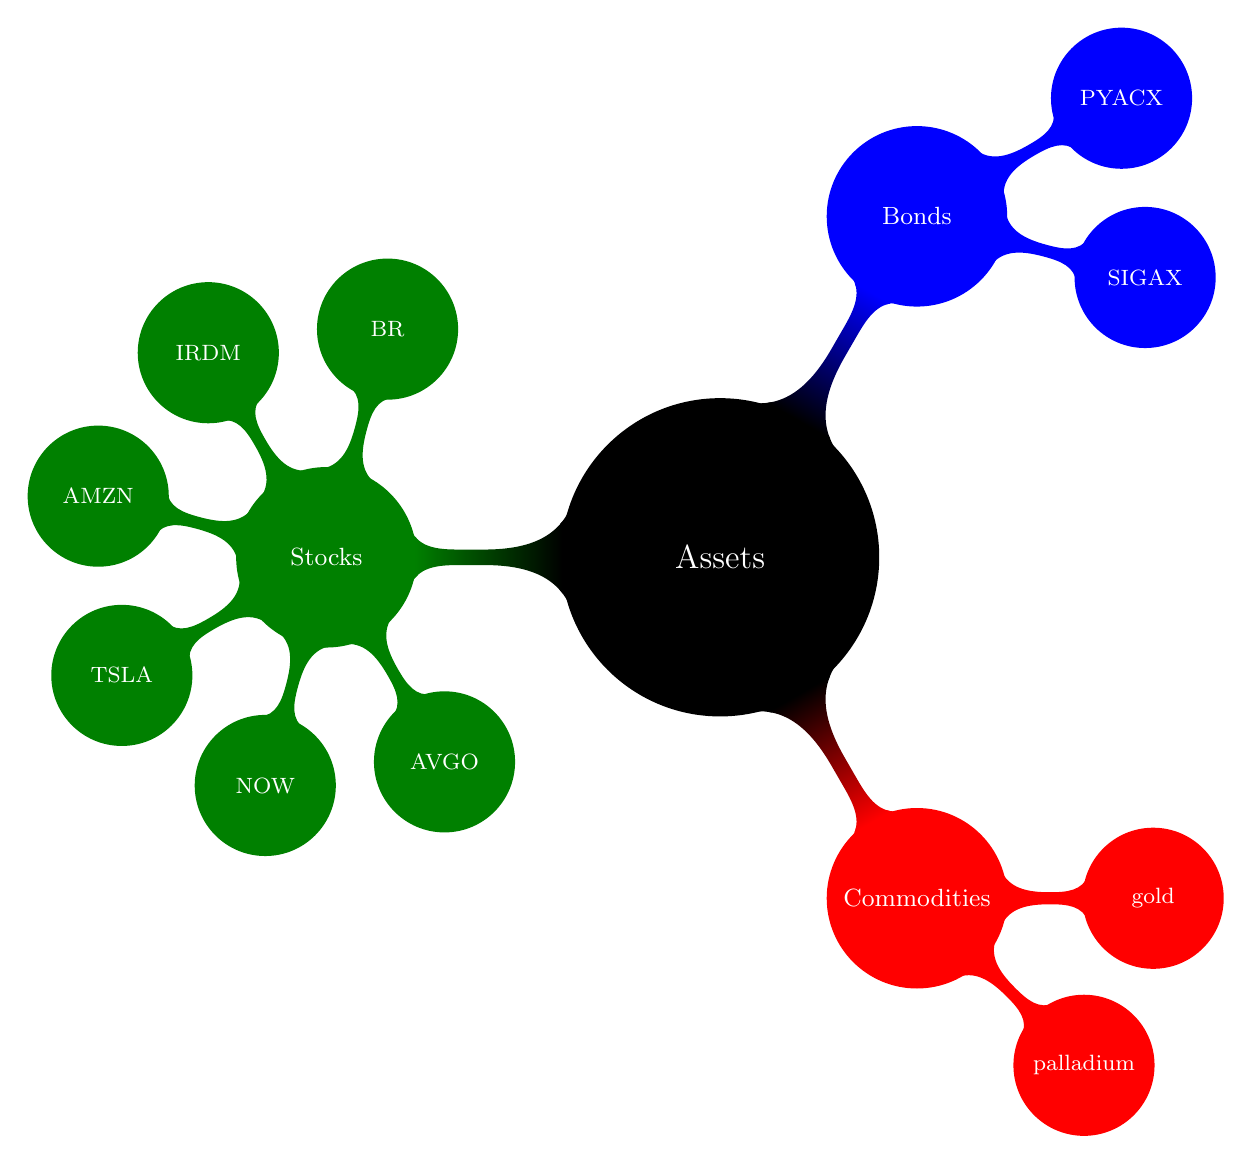
\begin{tikzpicture}[mindmap, grow cyclic, every node/.style=concept, concept color=black,text=white,
  level 1/.append style={level distance=5cm,sibling angle=120},
  level 2/.append style={level distance=3cm,sibling angle=45}]
  % ['AVGO', 'NOW', 'TSLA', 'AMZN', 'IRDM', 'BR', 'PYACX', 'SIGAX', 'gold', 'palladium', 'S&P 500']
  \node{Assets}
    [clockwise from=-180]
    child[concept color=green!50!black] {
      node[concept] {Stocks}
      [clockwise from=-60]
      child { node[concept] {AVGO} }
      child { node[concept] {NOW} }
      child { node[concept] {TSLA} }
      child { node[concept] {AMZN} }
      child { node[concept] {IRDM} }
      child { node[concept] {BR} }
      % child { node[concept] {pro\-gramming languages} }
      % child { node[concept] {software engineer\-ing} }
    }  
    child[concept color=blue] {
      node[concept] {Bonds}
      [clockwise from=30]
      child { node[concept] {PYACX} }
      child { node[concept] {SIGAX} }
    }
    child[concept color=red] {
      node[concept] {Commodities}
      [clockwise from=0]
      child { node[concept] {gold} }
      child { node[concept] {palladium} }
    }
    % child[concept color=red] { node[concept] {technical} }
    % child[concept color=orange] { node[concept] {theoretical} }
    ;
\end{tikzpicture}
\end{document}

% \usepackage[utf8]{inputenc}
% \usepackage{tikz}
% \usetikzlibrary{mindmap}

% \pagestyle{empty}
% \begin{document}

% \begin{tikzpicture}[mindmap, grow cyclic, every node/.style=concept, concept color=orange!40,
%     level 1/.append style={level distance=5cm,sibling angle=120},
%     level 2/.append style={level distance=3cm,sibling angle=45}]

% \node{ShareLaTeX Tutorial Videos}
%     child [concept color=blue!30] { node {Beginners Series}
%         child { node {First Document}}
%         child { node {Sections and Paragraphs}}
%         child { node {Mathematics}}
%         child { node {Images}}
%         child { node {bibliography}}
%         child { node {Tables and Matrices}}
%         child { node {Longer Documents}}
%     }
%     child [concept color=yellow!30] { node {Thesis Series}
%         child { node {Basic Structure}}
%         child { node {Page Layout}}
%         child { node {Figures, Subfigures and Tables}}
%         child { node {Biblatex}}
%         child { node {Title Page}}
%     }
%     % child [concept color=teal!40] { node {Beamer Series}
%     %     child { node {Getting Started}}
%     %     child { node {Text, Pictures and Tables}}
%     %     child { node {Blocks, Code and Hyperlinks}}
%     %     child { node {Overlay Specifications}}
%     %     child { node {Themes and Handouts}}
%     % }
%     child [concept color=purple!50] { node {TikZ Series}
%         child { node {Basic Drawing}}
%         child { node {Geogebra}}
%         child { node {Flow Charts}}
%         child { node {Circuit Diagrams}}
%         % child [concept color=green!40] { node {Mind Maps}}
%     };
% \end{tikzpicture}

% \end{document}